\documentclass[a4paper, 11pt]{article}
\usepackage[utf8]{inputenc} % Change according your file encoding
\usepackage{graphicx}
\usepackage{url}
\usepackage[margin=1in]{geometry}
\usepackage{caption}
\usepackage{subcaption}
\usepackage{float}

\usepackage[catalan,english]{babel}


%% Estil de Paràgraf
\setlength{\parskip}{4mm}
\setlength{\parindent}{0mm}

%% Estil lletra
\renewcommand{\familydefault}{\sfdefault}


%% Estil de Paràgraf
\setlength{\parskip}{4mm}
\setlength{\parindent}{0mm}

%opening
\title{Seminar Report: Chatty}
\author{Martín Garcia \and Ferran Arau}
\date{\today{}}

\begin{document}

\maketitle

\section{Introducció}

% Introduce in a couple of sentences the seminar and the main topic related to
% distributed systems it covers.

El seminari té com objectiu desenvolupar un sistema de ''chat'' distribuit
utilizant el paradigma client-servidor mitjançant events. Hi ha de dues
implementacions que cal desenvolupar.

En primer lloc els clients envien missatges a un únic servidor i aquest els
distribueix a la resta. 

En segon lloc, cal desenvolupar un sistema més robust ja que la primera
implementació presenta un únic punt de fallada crític, el servidor. Consisteix
en disposar de diverses instàncies ''Servidor'' i que aquestes es comuniquin
entre si. Els clients poden establir conexió amb qualsevol dels servidors i
aquests facilitaran els missatges rebuts a la resta de servidors propagant així
els missatges fins als clients últims.

\section{Feina de laboratori}

% Present the new code that you have added or how you have implemented a
% required functionality by using small Erlang code snippets (you do not need to
% copy\&paste all the code).

A continuació es presenten les dues implementacions del sistema de ''chat''. Es
mostren les diferències entre el codi original i el de producció mitjançant les
eines de ''history'' que proporciona el repositori utilitzat. 

Es pot consultar el codi d'aquesta sessió a
\url{https://github.com/magarcia/SDX/tree/master/S1}


\section{Experiments}

% Describe the experiments you did and provide evidence of the results you got
% (e.g., use screenshots). In addition, you may provide figures or tables with
% experimental results of the system evaluation. For each seminar, we will
% provide you with some guidance on which kind of evaluation you should do.

Per la primera implementació s'ha provat que el ''chat'' era funcional, és a
dir, s'ha vist que diversos clients es podien comunicar entre si. Tots els
clients poden veure tots els missatges.  També s'ha provat de deshabilitar el
servidor. Els resultats han estat els esperats, la comunicació entre els clients
s'ha vist afectada.

A continuació es mostren les imatges que corroboren les proves fetes.

\begin{center} 
	\textbf{Implementació 1}
\end{center}
\begin{figure}[H]
    \centering   
    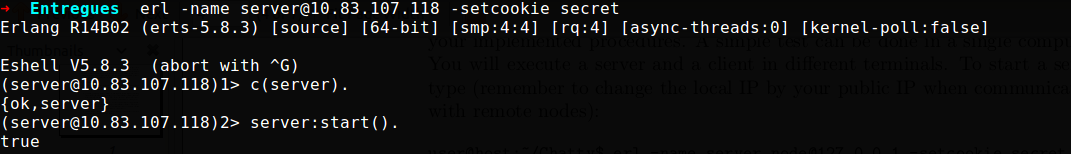
\includegraphics[width=0.8\textwidth]{figures/Server1_start}
    \caption{Servidor \label{fig:Impl1_Server}}    
\end{figure}
    
\begin{figure}[H]
    \centering   
	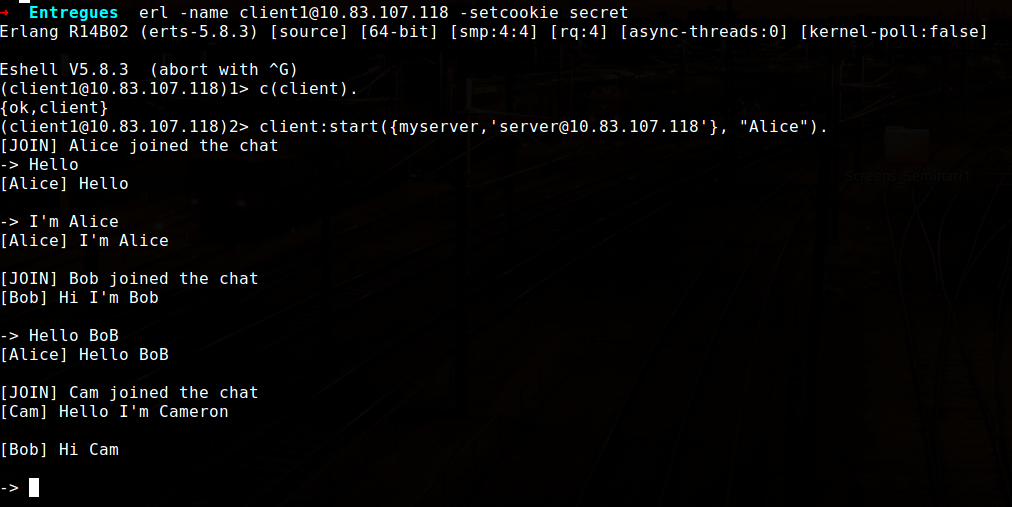
\includegraphics[width=0.8\textwidth]{figures/Server1_Al}
    \caption{Primer Client \label{fig:Impl1_Al}}	
\end{figure}

\begin{figure}[H]
    \centering   
	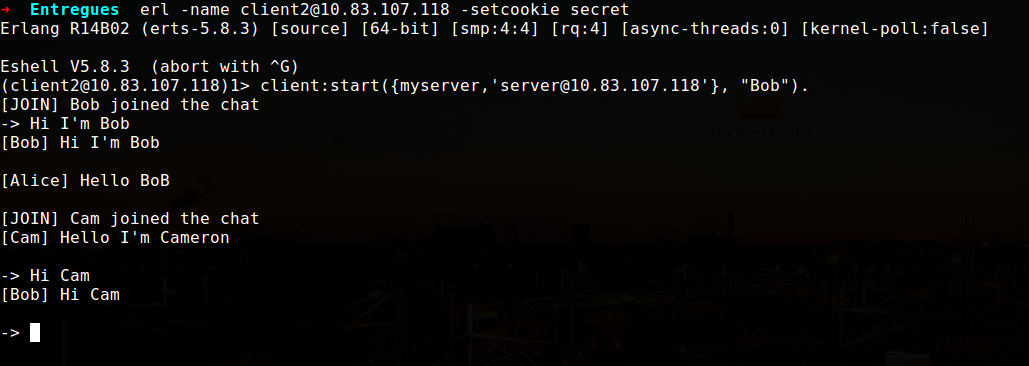
\includegraphics[width=0.8\textwidth]{figures/Server1_Bob}
    \caption{Segon Client \label{fig:Impl1_Bob}}    
\end{figure}    
    
\begin{figure}[H]
    \centering   
	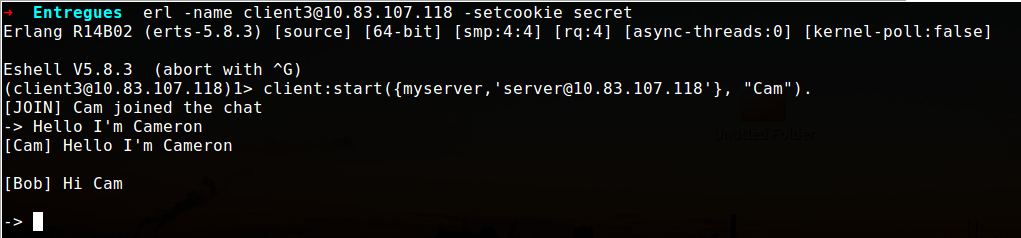
\includegraphics[width=0.8\textwidth]{figures/Server1_Cam}
    \caption{Tercer Client \label{fig:Impl1_Cam}}	
\end{figure}


Exemple de prova de la segona implementació amb 2 servidors:

\begin{figure}[H]
    \centering
    \begin{subfigure}[b]{0.8\textwidth}
        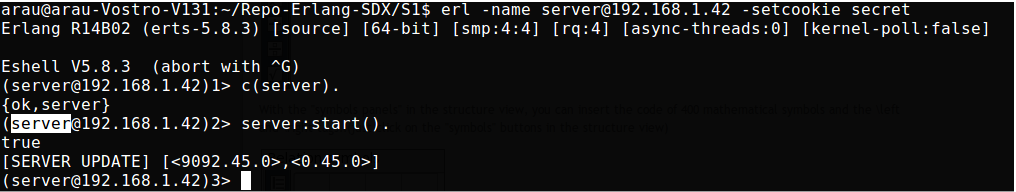
\includegraphics[width=1.0\textwidth]{figures/ServerA}
        \caption{Servidor primari}
        \label{fig:firstserver}
    \end{subfigure}
    
    \begin{subfigure}[b]{0.8\textwidth}
        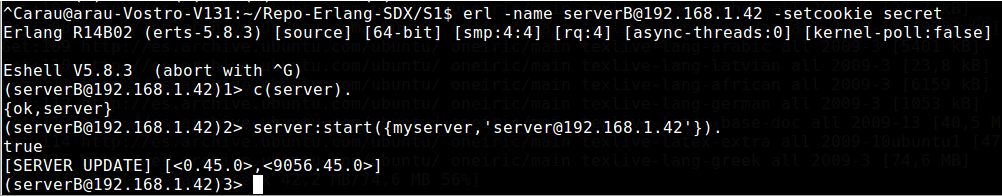
\includegraphics[width=1.0\textwidth]{figures/ServerB}
        \caption{Servidor secondari}
        \label{fig:secondserver}
    \end{subfigure}

    \begin{subfigure}[b]{0.8\textwidth}
        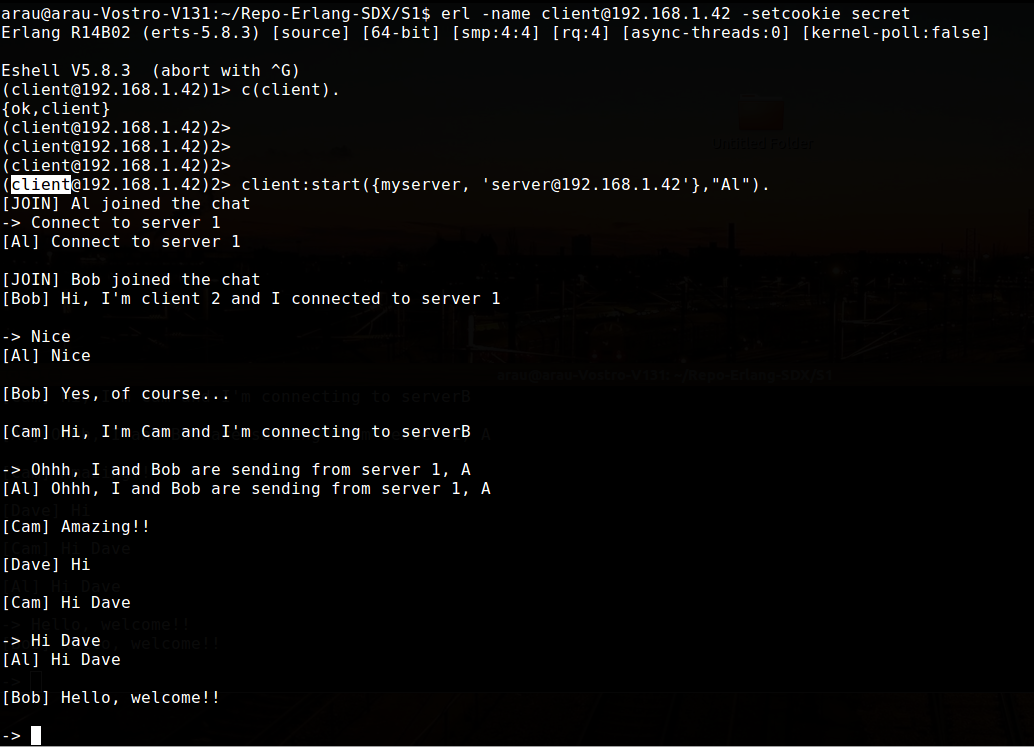
\includegraphics[width=1.0\textwidth]{figures/Al}
        \caption{Client 1}
        \label{fig:firstclient}
    \end{subfigure}

    \caption{Implementació 2}
\end{figure}

\begin{figure}[H]
    \centering
    
    \begin{subfigure}[b]{0.8\textwidth}
        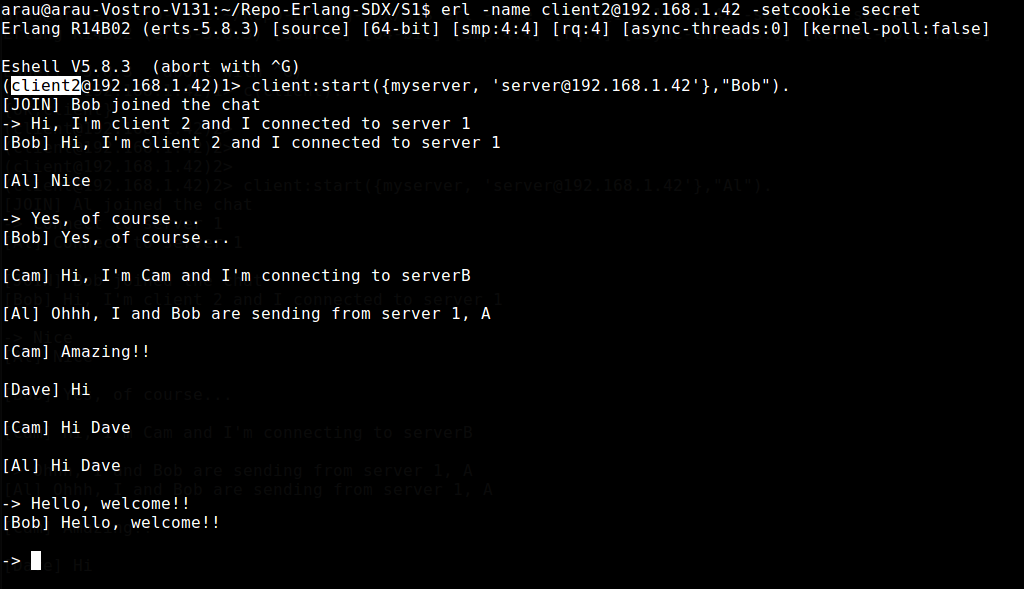
\includegraphics[width=1.0\textwidth]{figures/Bob}
        \caption{Client 2}
        \label{fig:secondserver}
    \end{subfigure}

    \begin{subfigure}[b]{0.8\textwidth}
        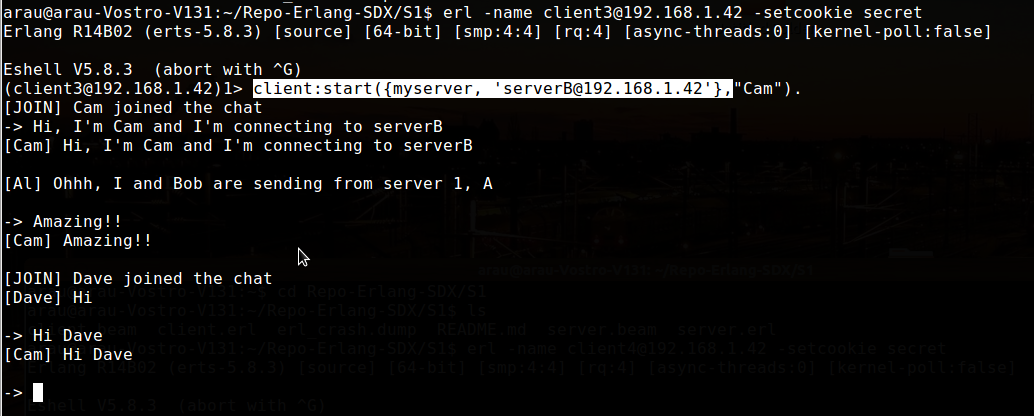
\includegraphics[width=1.0\textwidth]{figures/Cam}
        \caption{Client 3}
        \label{fig:thirdserver}
    \end{subfigure} 
        
    \begin{subfigure}[b]{0.8\textwidth}
        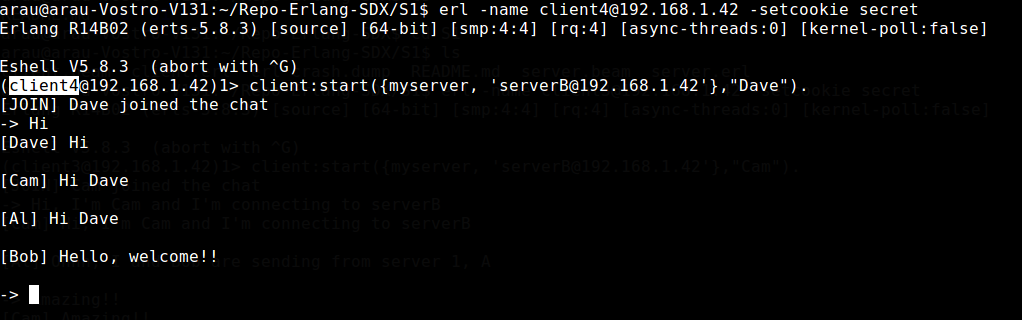
\includegraphics[width=1.0\textwidth]{figures/Dave}
        \caption{Client 4}
        \label{fig:fourthserver}
    \end{subfigure}    

\end{figure}

\section{Open questions}

% Try to answer all the open questions in the documentation. When possible, do
% experiments to support your answers.

\section{Personal Opinion}

% Your personal opinion of the seminar, including whether it should be included
% in next year's course or not.


\end{document}

